\begin{frame}
    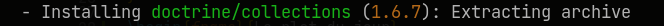
\includegraphics[width=\textwidth]{screenshots/Screenshot_20210520_104535.png}
\end{frame}

\begin{frame}
    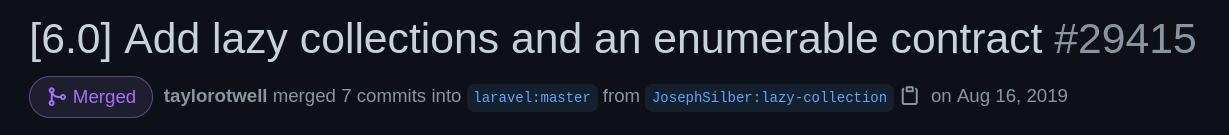
\includegraphics[width=\textwidth]{screenshots/Screenshot_20210520_101402.png}
    
\includegraphics[width=\textwidth]{screenshots/Screenshot_20210520_101458.png}
\end{frame}

\begin{frame}{Pourquoi}{Motivations}
    \begin{itemize}[<+->]
        \item \colorbox{yellow}{\textbf{Personnelles}}, envie d'apprendre et d'expérimentation, \textit{learning-by-doing}
        \item Aider à mieux \colorbox{yellow}{\textbf{comprendre}} les principes
        \item \colorbox{yellow}{\textbf{Simplifier}} l'utilisation de ces concepts
        \item \colorbox{yellow}{\textbf{Corriger}} un manquement (besoin $\Rightarrow$ solution)
    \end{itemize}
\end{frame}

\begin{frameC}{Pourtant, on a déjà tout en PHP!}{Etat des lieux}

\end{frameC}

\begin{frame}{Pourquoi}{Etat des lieux}
    PHP dispose de \colorbox{yellow}{\textbf{fonctions natives}} propices à l'itération

    \pause

    \begin{itemize}[<+->]
        \item Les fonctions \texttt{array\_*} (\textit{$\pm$ 52 disponibles})

        \begin{itemize}
            \item \texttt{array\_map()}
            \item \texttt{array\_filter()}
            \item \texttt{array\_reduce()}
            \item \texttt{array\_walk()}
        \end{itemize}
    \item \texttt{iterator\_to\_array()}
    \end{itemize}
\end{frame}

\begin{frame}{Pourquoi}{Etat des lieux}
    PHP dispose de \colorbox{yellow}{\textbf{structures natives}} propices à l'itération

    \pause

    \begin{itemize}[<+->]
        \item Tableaux (\texttt{array})
        \item Objects/Interfaces (\texttt{ArrayObject}, \texttt{ArrayAccess})
        \item Itérateurs
    \end{itemize}
\end{frame}

\begin{frame}{Pourquoi}{Etat des lieux}
    PHP dispose de \colorbox{yellow}{\textbf{structures natives}} propices à l'itération

    \pause

    \begin{itemize}[<+->]
        \item \texttt{for}
        \item \texttt{foreach}
        \item \texttt{while}
        \item \texttt{do-while}
    \end{itemize}
\end{frame}

\begin{frameC}{Oui, mais\ldots}

\end{frameC}

\begin{frame}{Pourquoi}{Des incohérences dans les fonctions}
    \begin{itemize}
        \item \texttt{array\_map()}
        \item \texttt{array\_filter()}
        \item \texttt{array\_reduce()}
        \item \texttt{array\_walk()}
        \item \ldots
    \end{itemize}
\end{frame}

\begin{frame}{Pourquoi}{Des incohérences dans les fonctions}
    \begin{itemize}[<+->]
        \item Uniquement pour les \texttt{array}
        \item Ordre des arguments (\textit{Sera probablement différent avec PHP 8})
        \begin{itemize}[<+->]
            \item \texttt{array\_map(\$callable, \$array)} ou \\ \texttt{array\_map(\$array, \$callable)} ?
            \item \texttt{array\_filter(\$callable, \$array)} ou \\ \texttt{array\_filter(\$array, \$callable)} ?
        \end{itemize}
        \item Inconsistance des paramètres (\texttt{callbacks})
        \item Pas de vérification des types
        \item Performances
    \end{itemize}
\end{frame}

\begin{frame}{Incohérences}{Exemple avec \texttt{array\_map()}}
    Un \texttt{array} est composé de \colorbox{yellow}{\textbf{couple(s)}} de\ldots

    \bigskip

    \begin{itemize}[<+->]
        \item<1-> Clé
        \visible<3->{
            \begin{itemize}[<+->]
                \item Unique
                \item Type \texttt{integer} ou \texttt{string} uniquement
            \end{itemize}
        }
        \item<2-> Valeur
        \visible<4->{
            \begin{itemize}[<+->]
                \item Pas de restrictions ni sur l'unicité, ni sur le typage
            \end{itemize}
        }

    \end{itemize}
\end{frame}

\begin{frameC}{Cependant\ldots}

\end{frameC}

\begin{frame}{Incohérences}{Exemple avec le célèbre \texttt{array\_map()}}
    \texttt{array\_map(callable \$callback, array \$data): array}

    \pause

    \begin{itemize}[<+->]
        \item \texttt{\$callback}

        \begin{itemize}[<+->]
            \item \texttt{callable} qui n'accepte qu'\colorbox{yellow}{\textbf{une seule}} valeur
        \end{itemize}

        \item \texttt{\$data}

        \begin{itemize}[<+->]
            \item N'accepte que les valeurs de type \colorbox{yellow}{\texttt{\textbf{array}}}
        \end{itemize}

        \item Retourne un \texttt{array}
    \end{itemize}

\end{frame}

\begin{frame}{Incohérences}{Exemple avec le célèbre \texttt{array\_map()}}
    \begin{itemize}[<+->]
        \item \colorbox{yellow}{\textbf{Pourquoi}} alors la clé n'est elle pas passée à \texttt{\$callback} ?
        \item \colorbox{yellow}{\textbf{Pourquoi}} cela ne fonctionne que pour les \texttt{array} ?
        \item \colorbox{yellow}{\textbf{Pourquoi}} \texttt{array\_filter()} nous permet de le faire ?
        \item \colorbox{yellow}{\textbf{Pourquoi}}\ldots
    \end{itemize}
\end{frame}

\begin{frame}
    \begin{center}
        \includegraphics[width=\textwidth]{meme/b5p0aqqs1qc51.png}
    \end{center}
\end{frame}

\begin{frameC}{Bref\ldots}

\end{frameC}

\begin{frame}{Pourquoi}{Bref\ldots}
    \begin{itemize}[<+->]
        \item On \colorbox{yellow}{\textbf{sait}} que PHP n'est pas parfait\ldots \pause[\thebeamerpauses] mais qu'il va bientôt l'être!\pause
        \item On a \colorbox{yellow}{\textbf{l'habitude}}\ldots \pause[\thebeamerpauses] et donc, on ne fait plus attention\pause
        \item Cela ne nous empêche pas de construire de \colorbox{yellow}{\textbf{belles choses}} malgré tout
    \end{itemize}
\end{frame}
